反之，把张量网络图翻译成数学表达式也可能得到多种解释。例如下面这个矩阵乘法图
$
\begin{tikzpicture}[baseline=\baseline]
   \tikzset{tensor/.style = {minimum size = 0.5cm,shape = circle,thick,draw=black,inner sep = 0pt}, edge/.style = {thick,line width=.4mm},every loop/.style={}}
    \def\y{0}
    \def\x{0}
    \node[tensor,fill=red!50!white] (A) at (\x,\y){\scalebox{0.85}{$\Ab$}};
    \node[tensor,fill=blue!50!white] (B) at (\x+1,\y){\scalebox{0.85}{$\Bb$}};
    \draw[edge] (A) -- (B) node [midway,above] {\scalebox{0.7}{\dimcolor{$R$}}};
    \draw[edge] (\x-0.25,\y) -- (\x-0.75,\y) node [midway,above] {\scalebox{0.7}{\dimcolor{$d_1$}}};
    \draw[edge] (\x+1.25,\y) -- (\x+1.75,\y) node [midway,above] {\scalebox{0.7}{\dimcolor{$d_2$}}};
\end{tikzpicture}
$
依据我们为 $\Ab$、$\Bb$ 与结果矩阵选定的形状不同，它有不同的解读：
\begin{itemize}
    \item 若 $\Ab\in\RR^{d_1\times R}, \Bb\in\RR^{R\times d_2}$ 且结果的大小为 $d_1 \times d_2$，则该图表示乘积 $\Ab\Bb$，
    \item 若 $\Ab\in\RR^{R\times d_1}, \Bb\in\RR^{R\times d_2}$ 且结果的大小为 $d_1 \times d_2$，则该图表示乘积 $\Ab^\ts\Bb$，
    \item 若 $\Ab\in\RR^{R\times d_1}, \Bb\in\RR^{R\times d_2}$ 且结果的大小为 $d_2 \times d_1$，则该图表示乘积 $\Bb^\ts\Ab$，
    \item ...
\end{itemize}
因此，把张量网络图翻译成数学表达式时要多加留心。但这也正是张量网络如此有用之处！当我们操作图示而非数学表达式时，就不必在意例如转置这样的问题。

\paragraph{收缩同一节点的两条腿。 } 如前所述，任意两条维度相同的腿都可以连接起来，构成张量网络中的一条边，即使它们属于同一个节点。举例来说，考虑五阶张量 $\Tt\in\mathbb R^{d_1\times d_2 \times d_3 \times d_2 \times d_4}$。它的第 2 个与第 4 个模维度相同，因此可以把二者收缩在一起。所得的张量网络有三条悬空腿，因而表示一个三阶张量： 
\begin{align*}
&\begin{tikzpicture}[baseline=-0.5ex]
    \tikzset{tensor/.style = {minimum width = 1.8cm,minimum height = 0.4cm,shape = rounded rectangle,thick,draw=black,inner sep = 0pt}, edge/.style = {thick,line width=.4mm},every loop/.style={}}
    \def\x{0}
    \def\y{0}
    \draw[edge] (\x-0.4,\y-0.15) -- (\x-0.4,\y-0.5)node [near end,left=-0.05cm] {\scalebox{0.7}{\dimcolor{$d_2$}}};
    \draw[edge] (\x-0.8,\y-0.15) -- (\x-0.8,\y-0.5)node [near end,left=-0.05cm] {\scalebox{0.7}{\dimcolor{$d_1$}}};
    \draw[edge] (\x,\y-0.15) -- (\x,\y-0.5)node [near end,left=-0.05cm] {\scalebox{0.7}{\dimcolor{$d_3$}}};
    \draw[edge] (\x+0.4,\y-0.15) -- (\x+0.4,\y-0.5)node [near end,left=-0.05cm] {\scalebox{0.7}{\dimcolor{$d_2$}}};
    \draw[edge] (\x+0.8,\y-0.15) -- (\x+0.8,\y-0.5)node [near end,left=-0.05cm] {\scalebox{0.7}{\dimcolor{$d_4$}}};
    \node[tensor,fill=green!30!white] (Bt) at (\x,\y){$\Tt$};
    \end{tikzpicture}\in \mathbb R^{d_1\times d_2\times d_3 \times d_2 \times d_4},\ \ \ \ 
  \begin{tikzpicture}[baseline=-0.5ex]
    \tikzset{tensor/.style = {minimum width = 1.8cm,minimum height = 0.4cm,shape = rounded rectangle,thick,draw=black,inner sep = 0pt}, edge/.style = {thick,line width=.4mm},every loop/.style={}}
    \def\x{0}
    \def\y{0}
    \draw[edge] (\x-0.4,\y-0.15) -- (\x-0.4,\y-0.5);
    \draw[edge] (\x-0.8,\y-0.15) -- (\x-0.8,\y-0.5)node [pos=1.3] {\scalebox{0.7}{\indcolor{$i_1$}}};
    \draw[edge] (\x,\y-0.15) -- (\x,\y-0.5)node [pos=1.3] {\scalebox{0.7}{\indcolor{$i_3$}}};
    \draw[edge] (\x+0.4,\y-0.15) -- (\x+0.4,\y-0.5);
    \draw[edge] (\x-0.4,\y-0.5) to [out=270,in=270] (\x+0.4,\y-0.5) node [midway,below=0.7cm] {\scalebox{0.7}{\dimcolor{$d_2$}}};
    \draw[edge] (\x+0.8,\y-0.15) -- (\x+0.8,\y-0.5)node[pos=1.3] {\scalebox{0.7}{\indcolor{$i_4$}}};
    \node[tensor,fill=green!30!white] (Bt) at (\x,\y){$\Tt$};
    \end{tikzpicture} = \sum_{i_2=1}^{d_2} \Tt_{i_1,i_2,i_3,i_2,i_4},   %
    \text{ and }\ \ \
    \begin{tikzpicture}[baseline=-0.5ex]
    \tikzset{tensor/.style = {minimum width = 1.8cm,minimum height = 0.4cm,shape = rounded rectangle,thick,draw=black,inner sep = 0pt}, edge/.style = {thick,line width=.4mm},every loop/.style={}}
    \def\x{0}
    \def\y{0}
    \draw[edge] (\x-0.4,\y-0.15) -- (\x-0.4,\y-0.5);
    \draw[edge] (\x-0.8,\y-0.15) -- (\x-0.8,\y-0.5)node [midway,left=-0.05cm] {\scalebox{0.7}{\dimcolor{$d_1$}}};
    \draw[edge] (\x,\y-0.15) -- (\x,\y-0.5)node [midway,left=-0.05cm] {\scalebox{0.7}{\dimcolor{$d_3$}}};
    \draw[edge] (\x+0.4,\y-0.15) -- (\x+0.4,\y-0.5);
    \draw[edge] (\x-0.4,\y-0.5) to [out=270,in=270] (\x+0.4,\y-0.5) node [midway,below=0.7cm] {\scalebox{0.7}{\dimcolor{$d_2$}}};
    \draw[edge] (\x+0.8,\y-0.15) -- (\x+0.8,\y-0.5)node [midway,left=-0.05cm] {\scalebox{0.7}{\dimcolor{$d_4$}}};
    \node[tensor,fill=green!30!white] (Bt) at (\x,\y){$\Tt$};
    \end{tikzpicture} \in \mathbb R^{d_1\times d_3 \times d_4}.
\end{align*}
收缩一个 $N$ 阶张量的两条腿后，所得张量的阶数为 $N-2$。这与后文将要介绍的\emph{偏迹}（partial trace）概念密切相关。
\subsection{内积、外积、迹与范数}\label{sec:inner-products}
本节借助张量网络说明，内积（inner product）、外积（outer product）、迹（trace）与范数（norm）这些经典概念如何推广到高阶张量。

\paragraph{内积} 与向量之间经典的内积~（欧几里得内积）类似，两个 $N$ 阶张量 $\St,\Tt\in\RR^{d_1\times\dots\times d_N}$ 的内积是它们对应元素乘积之和：
$$ \langle \St,\Tt \rangle = \sum_{i_1=1}^{d_1}\dots\sum_{i_N=1}^{d_N}\St_{i_1\dots i_N}\Tt_{i_1\dots i_N}.$$ 在张量网络图中，对所有维度求和就是把两个张量的所有腿都连接起来。这样得到的张量网络没有自由腿，表示一个标量。例如，对向量 $\ab\in\RR^{d\times 1}, \bb\in\RR^{d\times 1}$ 有
\begin{align}\label{eq:inner-product}
\langle\ab,\bb\rangle = \sum_{i=1}^d\ab_i\bb_i
=
    \begin{tikzpicture}[baseline=\baseline]
   \tikzset{tensor/.style = {minimum size = 0.5cm,shape = circle,thick,draw=black,inner sep = 0pt}, edge/.style = {thick,line width=.4mm},every loop/.style={}}
    \def\y{0}
    \def\x{0}
    \node[tensor,fill=red!30!white] (a) at (\x,\y){\scalebox{0.85}{$\ab$}};
    \node[tensor,fill=blue!30!white] (b) at (\x+1,\y){\scalebox{0.85}{$\bb$}};
    \draw[edge] (A) -- (B) node [midway,above]{\scalebox{0.7}{\dimcolor{$d$}}};
\end{tikzpicture},
\end{align}
对两个三阶张量 $\St,\Tt\in\RR^{d_1\times d_2\times d_3}$ 则有
\begin{align*}
\langle\St,\Tt\rangle = \sum_{i_1=1}^{d_1}\sum_{i_2=1}^{d_2}\sum_{i_3=1}^{d_3}\St_{i_1i_2i_3}\Tt_{i_1i_2i_3} =
\begin{tikzpicture}[baseline=\baseline]
    \tikzset{tensor/.style = {minimum size = 0.5cm,shape = circle,thick,draw=black,inner sep = 0pt}, edge/.style = {thick,line width=.4mm},every loop/.style={}}
    \def\y{0}
    \def\x{0}
    \node[tensor,fill=green!50!red!50!white] (St) at (\x,\y){\scalebox{0.85}{$\St$}};
    \node[tensor,fill=green!50!red!50!white] (Tt) at (\x+1,\y){\scalebox{0.85}{$\Tt$}};
    \draw[edge] (St) -- (Tt);
    \draw[edge] (St) to [out=45,in=135] (Tt);
    \draw[edge] (St) to [out=-45,in=-135] (Tt);
    \node[draw=none] () at (\x+0.5,\y+0.5) {\scalebox{0.7}{\dimcolor{$d_1$}}};
    \node[draw=none] () at (\x+0.5,\y+0.15) {\scalebox{0.7}{\dimcolor{$d_2$}}};
    \node[draw=none] () at (\x+0.5,\y-0.5) {\scalebox{0.7}{\dimcolor{$d_3$}}};
\end{tikzpicture}  
.
\end{align*}
本书只讨论实值张量，但张量网络这套形式语言稍加改造即可用于复值张量。
例如，若这两个张量取复值，就需对第二个张量的元素取共轭，这在张量网络中可以用节点 $\Tt^*$~（逐元素共轭）来代替 $\Tt$ 表示。
\paragraph{外积}\label{subsection:outer-product}
回忆一下，两个向量 $\ub\in\RR^{m},\vb\in\RR^n$ 的外积是 $m\times n$ 的秩一（rank-one）矩阵 $\ub\vb^\top$。
这一运算可推广到任意多个张量。例如，$N$ 个向量 $\ab_1\in\RR^{d_1},\cdots,\ab_N\in\RR^{d_N}$ 的外积是一个 $N$ 阶张量，其定义为
\begin{align*}
    (\ab_1 \outprod \ab_2 \outprod \cdots \outprod \ab_N)_{i_1,i_2,\cdots,i_n}
    &= \\
    &\hspace{-1cm}(\ab_1)_{i_1} (\ab_2)_{i_2}  \cdots (\ab_N)_{i_N}\ \text{for all } i_1 \in [d_1],\cdots, i_N\in[d_N].
\end{align*}
这样的张量称为\textbf{秩一}张量。 %
下图展示了 $N$ 个向量的外积： 
$$
\ab_1\outprod\ab_2 \outprod\cdots\outprod \ab_N=
\begin{tikzpicture}[baseline=\baseline]
    \tikzset{tensor/.style = {minimum size = 0.5cm,shape = circle,thick,draw=black,inner sep = 0pt}, edge/.style   = {thick,line width=.4mm}}
    \def\y{0}
     \def\x{0}
     \node[tensor,fill=blue!10!white] (a1) at (\x,\y){$\ab_1$};
    \node[tensor,fill=blue!10!white](a2) at (\x+1,\y){$\ab_2$};
  
    \node[tensor,fill=blue!10!white](an) at (\x+3,\y){$\ab_N$};
    \draw[edge] (a1) -- (\x,\y-0.7) node [midway, left] {\scalebox{0.7}{\dimcolor{$d_1$}}};
    \draw[edge] (a2) -- (\x+1,\y-0.7) node [midway, left] {\scalebox{0.7}{\dimcolor{$d_2$}}};
    \draw[edge] (an) -- (\x+3,\y-0.7)  node [midway, left] {\scalebox{0.7}{\dimcolor{$d_N$}}};
    \node (eq) at (\x+2,\y) {$\cdots$};
\end{tikzpicture}
\in\RR^{d_1\times\cdots\times d_N}.
$$
特别地，当 $N=2$ 时有  $\ab_1 \outprod \ab_2 = \ab_1\ab_2^\ts\in\RR^{d_1\times d_2}$。从外积的张量网络图中可以看到，节点之间没有共享边，这正对应于外积中不发生收缩（求和）。
外积的概念可以自然地推广到高阶张量。
设 $\At\in\RR^{m_1\times\dots\times m_p}$、$\Bt\in\RR^{n_1\times\dots\times n_q}$。$\At$ 与 $\Bt$ 的外积是一个 $p+q$ 阶张量，定义为 
$$ (\At\outprod\Bt)_{i_1,i_2,\cdots,i_p,j_1,j_2,\cdots,j_q} = \At_{i_1,i_2,\cdots,i_p} 
\Bt_{j_1,j_2,\cdots,j_q}. $$
与向量的情形一样，外积的张量网络只需把相应的节点并排摆放、不添加任何边即可得到：
$$
\At\outprod\Bt = 
   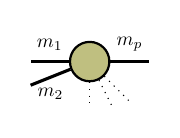
\begin{tikzpicture}[baseline=-0.5ex]
    \tikzset{tensor/.style = {minimum size = 0.5cm,shape = circle,thick,draw=black,inner sep = 0pt}, edge/.style = {thick,line width=.4mm},every loop/.style={}}
    \def\x{6}
    \node[tensor,fill=green!50!red!50!white] (A) at (\x,0) {$\At$};
    \draw[edge] (A) -- (\x-0.75,0) node [midway,above] {\scalebox{0.7}{\dimcolor{$m_1$}}};
    \draw[edge] (A) -- (\x+0.75,0) node [midway,above] {\scalebox{0.7}{\dimcolor{$m_p$}}};;
    \draw[edge] (A) -- (\x-0.75,-0.3) node [midway, below] {\scalebox{0.7}{\dimcolor{$m_2$}}};;
    \draw[dotted] (A) -- (\x,-0.6);
    \draw[dotted] (A) -- (\x+0.5,-0.5);
    \draw[dotted] (A) -- (\x+0.3,-0.6);
    \end{tikzpicture}
\hspace{0.3cm}
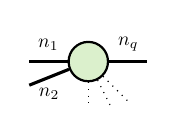
\begin{tikzpicture}[baseline=-0.5ex]
    \tikzset{tensor/.style = {minimum size = 0.5cm,shape = circle,thick,draw=black,inner sep = 0pt}, edge/.style = {thick,line width=.4mm},every loop/.style={}}
    \def\x{6}
    \def\y{0}
    \node[tensor,fill=green!70!red!20!white] (B) at (\x+1,\y) {$\Bt$};
    \draw[edge] (B) -- (\x+0.25,0) node [midway,above] {\scalebox{0.7}{\dimcolor{$n_1$}}};
    \draw[edge] (B) -- (\x+1.75,0) node [midway,above] {\scalebox{0.7}{\dimcolor{$n_q$}}};;
    \draw[edge] (B) -- (\x+0.25,-0.3) node [midway, below] {\scalebox{0.7}{\dimcolor{$n_2$}}};
    \draw[dotted] (B) -- (\x+1,-0.6);
    \draw[dotted] (B) -- (\x+1.5,-0.5);
    \draw[dotted] (B) -- (\x+1.3,-0.6);
\end{tikzpicture}\in\RR^{m_1\times\dots\times m_p\times n_1\times\dots\times n_q}.
$$
更一般地，对任意多个、阶数任意的张量，其外积的张量网络图只需把它们并排摆放即可得到。例如对  $\Tt\in\RR^{d_1\times d_2\times d_3 \times d_4}$、$\Ab\in\RR^{m\times n}$ 与 $\vb\in\RR^{p}$
$$
\Ab\outprod \Tt\outprod \vb
=
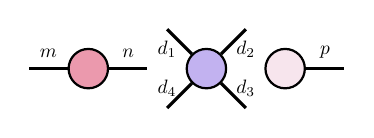
\begin{tikzpicture}[baseline=-0.5ex]
    \tikzset{tensor/.style = {minimum size = 0.5cm,shape = circle,thick,draw=black,inner sep = 0pt}, edge/.style = {thick,line width=.4mm},every loop/.style={}}
    \def\x{0}
    \def\y{0}
    \node[tensor,fill=blue!20!red!40!white] (A) at (\x,\y) {$\Ab$};
    \draw[edge] (A) -- (\x+0.75,\y)node [midway, above] {\scalebox{0.7}{\dimcolor{$n$}}};
    \draw[edge] (A) -- (\x-0.75,\y)node [midway, above] {\scalebox{0.7}{\dimcolor{$m$}}};
    \node[tensor,fill=red!20!blue!30!white] (T) at (\x+1.5,\y) {$\Tt$};
    \node[tensor,fill=red!70!blue!10!white] (v) at (\x+2.5,\y) {$\vb$};
    \draw[edge](T) -- (\x+2,\y-0.5);
    \node[draw=none] () at (\x+2,\y-0.25) {\scalebox{0.7}{\dimcolor{$d_3$}}};
    \draw[edge](T) -- (\x+2,\y+0.5);
    \node[draw=none] () at (\x+2,\y+0.25) {\scalebox{0.7}{\dimcolor{$d_2$}}};
    \draw[edge](T) -- (\x+1,\y-0.5);
    \node[draw=none] () at (\x+1,\y-0.25) {\scalebox{0.7}{\dimcolor{$d_4$}}};
    \draw[edge](T) -- (\x+1,\y+0.5);
    \node[draw=none] () at (\x+1,\y+0.25) {\scalebox{0.7}{\dimcolor{$d_1$}}};
    \draw[edge](v) -- (\x+3.25,\y)node [midway, above] {\scalebox{0.7}{\dimcolor{$p$}}};
\end{tikzpicture}\in\RR^{m\times n \times d_1\times d_2\times d_3 \times d_4\times p},
$$
其逐元素定义为 $(\Ab\outprod\Tt\outprod \vb)_{i_1i_2j_1j_2j_3j_4k} = \Ab_{i_1i_2}\Tt_{j_1\cdots j_4}\vb_{k}$，其中对 $l\in[4]$ 有 $i_1\in[m],i_2\in[n],j_l\in[d_l]$，且 $k\in[p]$。

